\subsection[Agrégation des sorties des couches]{Agrégation des sorties des couches~: d'une stratégie additive à une concaténation}\label{subsec:addcat_}
La première optimisation à été de changer la façon de regrouper les informations de toues les \og échelles\fg{} avant de les transmettre au module produisant la distribution de probabilité.

Initialement, les sorties de toutes les \og échelles\fg{} étaient sommées. Cela permettait de maintenir des \glspl{tensor} de dimensions uniformes quel que soit le nombre d'\og échelle\fg{} (\autoref{fig:add}).

Après discussion avec notre maître de stage, la stratégie d'agrégation à été changé en une concaténation des sorties.

Comme montré dans la \autoref{fig:cat}, la taille du \gls{tensor} concaténé change en fonction du nombre d'entrées.
La manipulation de \glspl{tensor} de taille non fixée est très ardue dans ce cas précis, bien que nous ne développerons pas plus avant les raisons de cette difficulté.

Cela à nécessité l'abandon de la propriété de croissance à l'infini de l'architecture (décrite \autoref{inf_growth}), au profit d'un nombre maximal d'échelles défini à l'avance ou déterminée à l'aide d'une formule en fonction des données disponibles (décrite \autoref{growth_formula}).

\begin{figure}[ht]
	\begin{subfigure}{0.45\textwidth}
		\centering
		\scalebox{1}{\def\layersep{5em}
\begin{tikzpicture}[shorten >=1pt,->,draw=black, node distance=\layersep]
\tikzstyle{every pin edge}=[<-,shorten <=1pt]
\tikzstyle{block}=[minimum size=2em];
\tikzstyle{value}=[rectangle, fill=green!50,block];
\tikzstyle{operation}=[block, circle,inner sep=0pt, fill=red!50];
\tikzstyle{nonlinearity}=[rectangle,block, fill=blue!50];
\tikzstyle{annot} = [text width=6em, text centered]

% Draw the input layer nodes
\foreach \name / \y in {1,...,3}
% This is the same as writing \foreach \name / \y in {1/1,2/2,3/3,4/4}
\node[value, label={[]north:{\'{E}chelle \y}}] (I-\name) at (0,-2*\y) {\y};
\node[value, label={[]north:{\'{E}chelle 4}}, opacity=.5] (I-4) at (0,-8) {4};

% Draw the output layer node
\node[operation, right of=I-2] (ope) {{\Large +}};
\node[value, right of=ope, label={[]north:$1+2+3+4$}](cat){};
% Draw the output layer node
%\node[nonlinearity, right of=cat] (lin) {Lin};
%\node[annot, right of=lin, text width=7em,xshift=2em ] (out) {Distribution de probabilit\'{e}s};

% Connect every node in the input layer with every node in the
% hidden layer.
\foreach \source in {1,...,3}
\path (I-\source.east) edge (ope);
\path (I-4.east) edge[dashed, opacity=.5] (ope);
\path (ope) edge (cat);
%\path (cat) edge (lin);
%\path (lin) edge (out);
\end{tikzpicture}}
		\caption[Stratégie d'agrégation additive]{Stratégie d'agrégation additive.\vspace{2.5em}}\label{fig:add}
	\end{subfigure}
	\begin{subfigure}{0.45\textwidth}
		\centering
		\scalebox{1}{\def\layersep{5em}
\begin{tikzpicture}[shorten >=1pt,->,draw=black, node distance=\layersep]
    \tikzstyle{every pin edge}=[<-,shorten <=1pt]
    \tikzstyle{block}=[minimum size=2em];
    \tikzstyle{value}=[rectangle, fill=green!50,block];
    \tikzstyle{operation}=[block, circle,inner sep=0pt, fill=red!50];
    \tikzstyle{nonlinearity}=[rectangle,block, fill=blue!50];
    \tikzstyle{annot} = [text width=6em, text centered]

    % Draw the input layer nodes
    \foreach \name / \y in {1,...,3}
    % This is the same as writing \foreach \name / \y in {1/1,2/2,3/3,4/4}
        \node[value, label={[]north:{\'{E}chelle \y}}] (I-\name) at (0,-2*\y) {\y};
	\node[value, label={[]north:{\'{E}chelle 4}}, opacity=.5] (I-4) at (0,-8) {4};

    % Draw the output layer node
    \node[operation, right of=I-2] (ope) {Cat};
    \node[value, right of=ope](cat){2};
    \node[value, above of=cat, node distance=2.1em]{1};
    \node[value, below of=cat, node distance=2.1em](3){3};
    \node[value, below of=3, node distance=2.1em, opacity=.5]{4};
    % Draw the output layer node
    \node[nonlinearity, right of=cat] (lin) {Lin};
	\node[annot, right of=lin, text width=7em,xshift=2em ] (out) {Distribution de probabilit\'{e}s};

    % Connect every node in the input layer with every node in the
    % hidden layer.
    \foreach \source in {1,...,3}
        \path (I-\source.east) edge (ope);
	\path (I-4.east) edge[dashed, opacity=.5] (ope);
	\path (ope) edge (cat);
	\path (cat) edge (lin);
	\path (lin) edge (out);
\end{tikzpicture}}
		\caption[Stratégie d'agrégation par concaténation]{Stratégie d'agrégation par concaténation. Les sorties sont mises côte-à-côte affin de former un nouveau \gls{tensor}.}\label{fig:cat}
	\end{subfigure} 
	\caption{Stratégies d'agrégation}
\end{figure}

La stratégie par concaténation est plus lente en terme de temps de calcul que la stratégie additive, cependant pour le même temps de calcul elle permet d'obtenir de meilleurs résultats (\autoref{fig:addcat}).

Voir l'annexe \ref{subsec:addcat} pour plus de détail sur le choix de la stratégie d'agrégation. 

\begin{figure}[H]
	\centering
	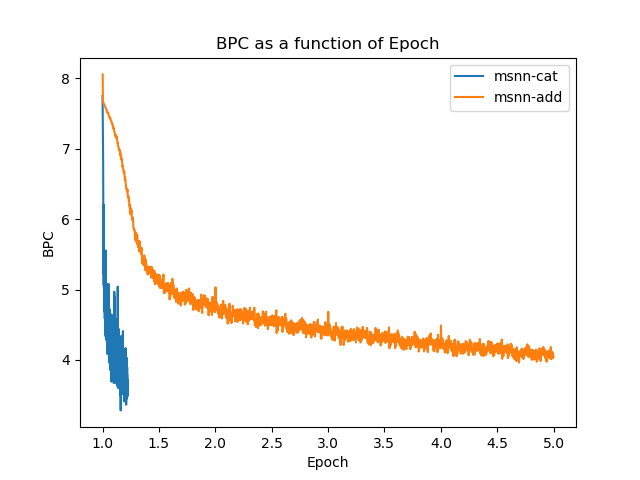
\includegraphics[width=\textwidth]{parts/appendix/reports-gmsnn/docs_esteban-latex/test_reports/comparative-bpc-msnn-det-msnn-cat.png}
	\caption[Performances comparées des stratégies additive et par concaténation]{Performances comparées des stratégies par concaténation (msnn-cat) et additive (msnn-add). Le temps de calcul alloué est identique. Avec la concaténation on entraîne le modèle sur 1/4 des données, avec l'addition on l'entraîne 5 fois sur l'ensemble des données. Avec la concaténation, on obtient une BPC de 3.5, alors qu'on obtient une BPC de 4 avec l'addition.}\label{fig:addcat}
\end{figure}